\begin{enumerate}[label=\thesubsection.\arabic*, ref=\thesubsection.\theenumi]

\item The sum of the following infinite series is:
\begin{align}
\frac{1}{1!} + \frac{1}{2!} + \frac{1}{3!} + \frac{1}{4!} + \frac{1}{5!} + \cdots
\end{align}
\hfill (GATE~BT~2025)
\begin{enumerate}
    \item $\pi$
    \item $1+e$
    \item $e-1$
    \item $e$
\end{enumerate}

\solution
From the Maclaurin series expansion of $e^x$ given in \eqref{eq:exp_maclaurin}:
\begin{align}
e^x = 1 + \frac{x}{1!} + \frac{x^2}{2!} + \frac{x^3}{3!} + \frac{x^4}{4!} + \cdots
\end{align}

Evaluating the expression at $x = 1$:
\begin{align}
e^1 &= 1 + \frac{1^1}{1!} + \frac{1^2}{2!} + \frac{1^3}{3!} + \frac{1^4}{4!} + \cdots \\
e &= 1 + \frac{1}{1!} + \frac{1}{2!} + \frac{1}{3!} + \frac{1}{4!} + \cdots \quad \brak{\text{since } 1^n = 1}
\end{align}

Using the original equation:
\begin{align}
\frac{1}{1!} + \frac{1}{2!} + \frac{1}{3!} + \frac{1}{4!} + \cdots = \sum_{n=1}^{\infty} \frac{1}{n!} \\ 
\implies \sum_{n=0}^{\infty} \frac{1}{n!} - 1 &= e - 1
\end{align}
Hence, option (C) is correct.

The following C code verifies the series sum numerically:

\begin{lstlisting}[frame=single, basicstyle=\rmfamily, escapeinside={(*@}{@*)}]
(*@\makebox[\dimexpr\linewidth-2\fboxsep-2\fboxrule\relax][c]{codes/btq3.c}@*)
\end{lstlisting}

\item A circle with center at $\brak{x, y} = \brak{0.5, 0}$ and radius $r_1 = 0.5$ intersects with another circle with center at $\brak{x, y} = \brak{1, 1}$ and radius $r_2 = 1$ at two points. One of the points of intersection $\brak{x, y}$ is:
\hfill (GATE~BT~2025)
\begin{enumerate}
    \item $\brak{0, 0}$
    \item $\brak{0.2, 0.4}$
    \item $\brak{0.5, 0.5}$
    \item $\brak{1, 2}$
\end{enumerate}

\solution
The matrix parameters for the two circles are formulated from their center vectors $\vec{c}_i$ and radii $r_i$:
\begin{align}
\text{Circle 1: } \vec{c}_1 = \myvec{0.5 \\ 0}, \; r_1 = 0.5 &\implies \vec{V}_1 = \vec{I} = \myvec{1 & 0 \\ 0 & 1}, \; \vec{u}_1 = -\vec{c}_1 = \myvec{-0.5 \\ 0} \\
f_1 &= \norm{\vec{c}_1}^2 - r_1^2 = 0.5^2 - 0.5^2 = 0 \\
\text{Circle 2: } \vec{c}_2 = \myvec{1 \\ 1}, \; r_2 = 1 &\implies \vec{V}_2 = \vec{I} = \myvec{1 & 0 \\ 0 & 1}, \; \vec{u}_2 = -\vec{c}_2 = \myvec{-1 \\ -1} \\
f_2 &= \norm{\vec{c}_2}^2 - r_2^2 = \brak{1^2 + 1^2} - 1^2 = 1
\end{align}

Using the pencil of conics from \eqref{eq:pencil_conics}, the condition for a degenerate conic from \eqref{eq:pencil_det_zero} gives:
\begin{align}
\det \myvec{\vec{V}_1 + \mu \vec{V}_2 & \vec{u}_1 + \mu \vec{u}_2 \\ \brak{\vec{u}_1 + \mu \vec{u}_2}^\top & f_1 + \mu f_2} = 0
\end{align}
Substituting the parameter matrices:
\begin{align}
\begin{vmatrix}
1 + \mu & 0 & -0.5 - \mu \\
0 & 1 + \mu & -\mu \\
-0.5 - \mu & -\mu & \mu
\end{vmatrix} = 0
\end{align}
Expanding the determinant:
\begin{align}
\brak{\ + \mu}\sbrak{\brak{1 + \mu}\mu - \mu^2} - \brak{-0.5 - \mu}\sbrak{0 - \brak{1 + \mu}\brak{-0.5 - \mu}} &= 0 \\
\brak{1 + \mu}\mu - \brak{1 + \mu}\brak{\mu + 0.5}^2 &= 0 \\
\brak{1 + \mu}\brak{-\mu^2 - \frac{1}{4}} &= 0
\end{align}
Since $\mu^2 + \frac{1}{4} = 0$ yields imaginary roots, the only real root is:
\begin{align}
\mu = -1
\end{align}

Substituting $\mu = -1$ into \eqref{eq:pencil_conics} eliminates the second-degree terms $\brak{\vec{V}_1 - \vec{V}_2 = \vec{0}}$, yielding the common chord (radical axis):
\begin{align}
2\brak{\vec{u}_1 - \vec{u}_2}^\top \vec{x} + \brak{f_1 - f_2} &= 0 \\
2\brak{\myvec{-0.5 \\ 0} - \myvec{-1 \\ -1}}^\top \vec{x} + \brak{0 - 1} &= 0 \\
2\myvec{0.5 & 1}\vec{x} - 1 = 0 \implies \myvec{1 & 2}\vec{x} &= 1
\end{align}
Thus, the equation of the line passing through the intersection points is $x + 2y = 1$.

The normal vector of this line is $\vec{n} = \myvec{1 \\ 2}$. A direction vector $\vec{m}$ orthogonal to $\vec{n}$ ($\vec{m}^\top \vec{n} = 0$) and a point $\vec{h}$ on the line are:
\begin{align}
\vec{m} = \myvec{2 \\ -1}, \quad \vec{h} = \myvec{1 \\ 0}
\end{align}
Expressing the line in parametric form $\vec{x} = \vec{h} + \kappa \vec{m}$ and substituting into Circle 1 using \eqref{eq:conic_kappa_roots}:
\begin{align}
\vec{m}^\top \vec{V}_1 \vec{m} &= \myvec{2 & -1}\myvec{1 & 0 \\ 0 & 1}\myvec{2 \\ -1} = 5 \\
\vec{V}_1 \vec{h} + \vec{u}_1 &= \myvec{1 \\ 0} + \myvec{-0.5 \\ 0} = \myvec{0.5 \\ 0} \\
\vec{m}^\top \brak{\vec{V}_1 \vec{h} + \vec{u}_1} &= \myvec{2 & -1}\myvec{0.5 \\ 0} = 1 \\
g\brak{\vec{h}} &= \vec{h}^\top \vec{V}_1 \vec{h} + 2\vec{u}_1^\top \vec{h} + f_1 = 1 - 1 + 0 = 0
\end{align}
Evaluating the parameter roots $\kappa$:
\begin{align}
\kappa = \frac{-1 \pm \sqrt{1^2 - 0}}{5} = \frac{-1 \pm 1}{5} \implies \kappa_1 = 0, \quad \kappa_2 = -\frac{2}{5}
\end{align}

The points of intersection are:
\begin{align}
\vec{x}_1 &= \vec{h} + 0\vec{m} = \myvec{1 \\ 0} \\
\vec{x}_2 &= \vec{h} - \frac{2}{5}\vec{m} = \myvec{1 \\ 0} - \frac{2}{5}\myvec{2 \\ -1} = \myvec{0.2 \\ 0.4}
\end{align}
Hence, one of the points of intersection is $\brak{0.2, 0.4}$, and option (B) is correct.


\begin{figure}[H]
    \centering
    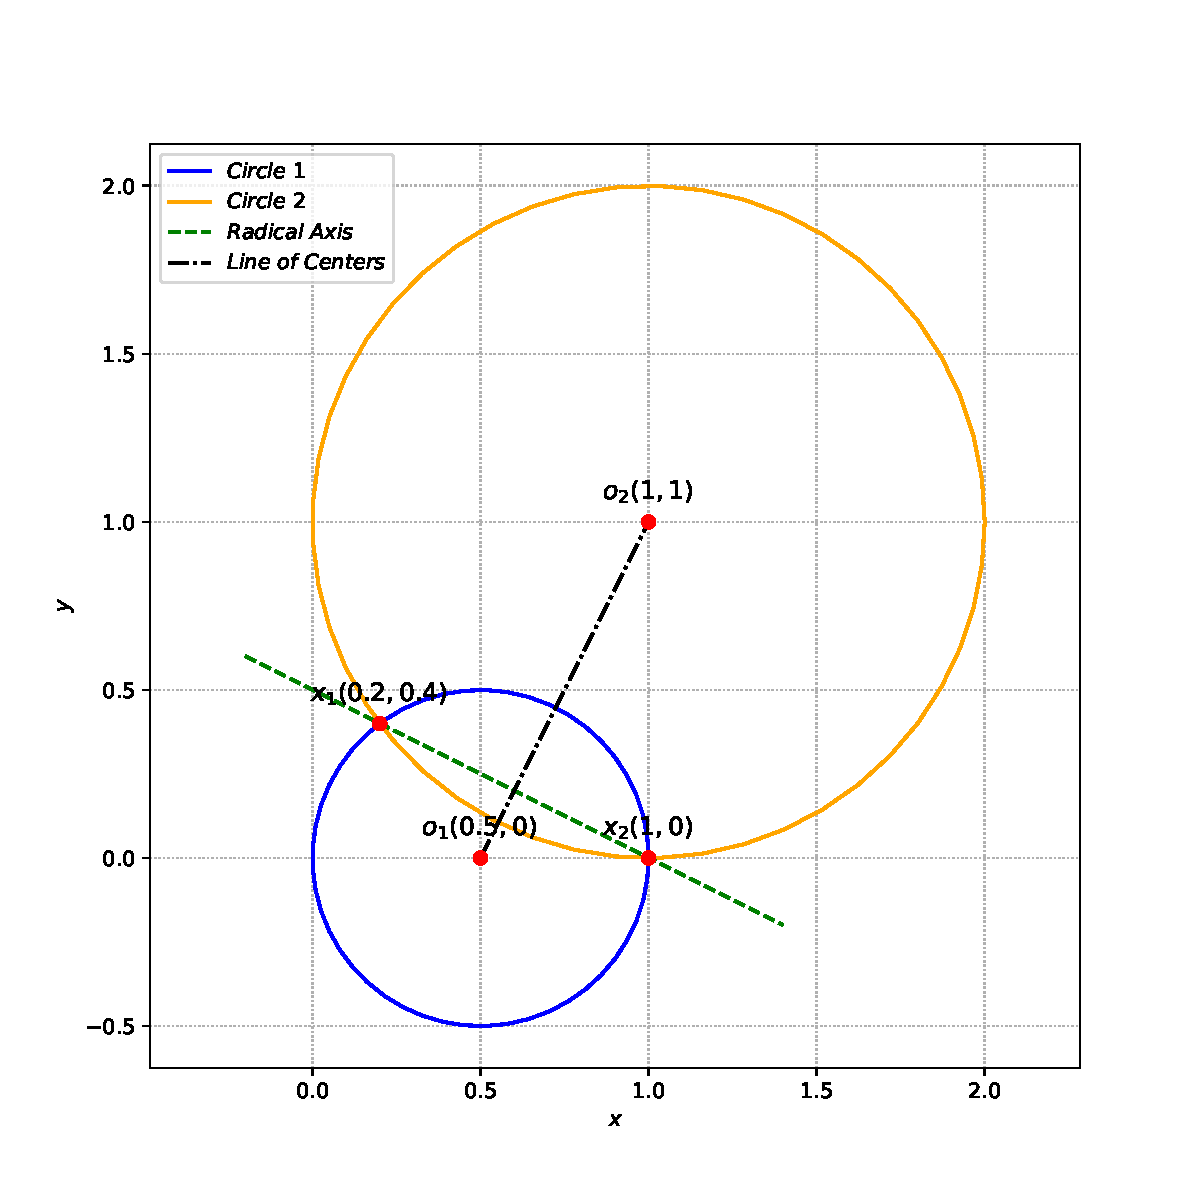
\includegraphics[width=0.70\linewidth]{figs/circleintersect.pdf}
    \caption{Intersection of the two circles and the radical axis}
    \label{fig:bt25_q9}
\end{figure}

\begin{lstlisting}[frame=single, basicstyle=\rmfamily, escapeinside={(*@}{@*)}]
(*@\makebox[\dimexpr\linewidth-2\fboxsep-2\fboxrule\relax][c]{codes/btq9/circleProblem1.py}@*)
\end{lstlisting}

\begin{lstlisting}[frame=single, basicstyle=\rmfamily, escapeinside={(*@}{@*)}]
(*@\makebox[\dimexpr\linewidth-2\fboxsep-2\fboxrule\relax][c]{figs/circleintersect.pdf}@*)
\end{lstlisting}

\item Let $y\brak{t}$ be a bacterial population whose growth is given by:
\begin{align}
\frac{dy}{dt} = \lambda\brak{y + 2}
\end{align}
where $\lambda$ is the growth rate constant. If $y\brak{0} = 1$ and $y\brak{1} = 4$, then the value of $\lambda$ is:
\hfill (GATE~BT~2025)
\begin{enumerate}
    \item $\ln 2$
    \item $\ln 3$
    \item $\ln 4$
    \item $\ln 6$
\end{enumerate}

\solution
Rearranging the differential equation into standard linear form:
\begin{align}
\frac{dy}{dt} - \lambda y = 2\lambda
\end{align}

Taking the unilateral Laplace transform on both sides using \eqref{eq:laplace_first_deriv} and \eqref{eq:laplace_const}:
\begin{align}
s Y(s) - y\brak{0} - \lambda Y(s) &= \frac{2\lambda}{s}
\end{align}


Substituting the initial condition $y\brak{0} = 1$:
\begin{align}
\brak{s - \lambda}Y(s) - 1 &= \frac{2\lambda}{s} \\
\brak{s - \lambda}Y(s) &= 1 + \frac{2\lambda}{s} = \frac{s + 2\lambda}{s} \\
Y(s) &= \frac{s + 2\lambda}{s\brak{s - \lambda}}
\end{align}

Decomposing into partial fractions:
\begin{align}
\frac{s + 2\lambda}{s\brak{s - \lambda}} = \frac{A}{s} + \frac{B}{s - \lambda} \implies s + 2\lambda = A\brak{s - \lambda} + B s
\end{align}

\item Evaluating the coefficients:
\begin{align}
\text{At } s = 0: \quad 2\lambda &= A\brak{-\lambda} \implies A = -2 \\
\text{At } s = \lambda: \quad 3\lambda &= B\brak{\lambda} \implies B = 3
\end{align}

Substituting $A$ and $B$ back into $Y(s)$ and applying the inverse Laplace transform using \eqref{eq:laplace_const} and \eqref{eq:laplace_exp_inv}:
\begin{align}
Y(s) &= -\frac{2}{s} + \frac{3}{s - \lambda} \\
y\brak{t} &= 3e^{\lambda t} - 2
\end{align}

Applying the boundary condition $y\brak{1} = 4$:
\begin{align}
4 &= 3e^{\lambda\brak{1}} - 2 \\
6 &= 3e^{\lambda} \\
e^{\lambda} &= 2 \implies \lambda = \ln 2
\end{align}
Hence, option (A) is correct.

\noindent{Numerical Simulation (Euler's Method):} \\
Applying the recurrence relation from \eqref{eq:euler_recurrence} with step size $h = 0.01$ and $\lambda = \ln 2$:
\begin{align}
y_{n+1} = y_n + 0.01\sbrak{\ln\brak{2}\brak{y_n + 2}}, \quad y_0 = 1
\end{align}

The C code implementation is as follows:

\begin{lstlisting}[frame=single, basicstyle=\rmfamily, escapeinside={(*@}{@*)}]
(*@\makebox[\dimexpr\linewidth-2\fboxsep-2\fboxrule\relax][c]{codes/btq13/bac.c}@*)
\end{lstlisting}


\begin{figure}[H]
    \centering
    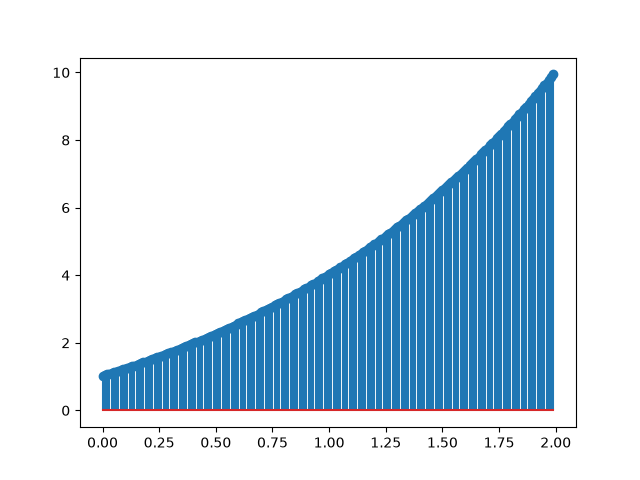
\includegraphics[width=0.70\linewidth]{figs/bac.png}
    \caption{Euler's Forward Difference Simulation of Bacterial Growth}
    \label{fig:bt25_q13}
\end{figure}

\begin{lstlisting}[frame=single, basicstyle=\rmfamily, escapeinside={(*@}{@*)}]
(*@\makebox[\dimexpr\linewidth-2\fboxsep-2\fboxrule\relax][c]{codes/btq13/bac.py}@*)
\end{lstlisting}


\begin{lstlisting}[frame=single, basicstyle=\rmfamily, escapeinside={(*@}{@*)}]
(*@\makebox[\dimexpr\linewidth-2\fboxsep-2\fboxrule\relax][c]{figs/bac.png}@*)
\end{lstlisting}

\item The minimum value of the function:
\begin{align}
f\brak{x} = x + \frac{4}{x}
\end{align}
for $x > 0$ is:
\hfill (GATE~BT~2025)
\begin{enumerate}
    \item $1$
    \item $2$
    \item $3$
    \item $4$
\end{enumerate}

\solution
To locate the critical points of $f\brak{x}$, we set the first derivative to zero:
\begin{align}
f'\brak{x} &= \diff{}{x}\brak{x + \frac{4}{x}} = 1 - \frac{4}{x^2} = 0 \\
1 &= \frac{4}{x^2} \implies x^2 = 4
\end{align}
Since $x > 0$, the only admissible critical point is:
\begin{align}
x = 2
\end{align}

Checking the second derivative using \eqref{eq:convexity_check}:
\begin{align}
f''\brak{x} = \frac{d^2}{dx^2}\brak{x + \frac{4}{x}} = \frac{8}{x^3}
\end{align}
For all $x \in \brak{0, \infty}$, $f''\brak{x} > 0$. Thus, $f\brak{x}$ is strictly convex, and $x = 2$ corresponds to a unique global minimum.

Evaluating the function at $x = 2$:
\begin{align}
f\brak{2} = 2 + \frac{4}{2} = 4
\end{align}
Hence, option (D) is correct.

\noindent{Numerical Simulation (Gradient Descent):} \\
Applying the first-order update relation from \eqref{eq:grad_descent_update} with learning rate $\eta = 0.3$:
\begin{align}
x_{k+1} = x_k - 0.3\brak{1 - \frac{4}{x_k^2}}
\end{align}
Starting from the initial guess $x_0 = 5$, the sequence converges to $x^* = 2$, yielding $f\brak{x^*} = 4$.

\item Alternative Method (Completing the Square):
For $x > 0$, the function $f\brak{x}$ can be expressed in terms of square roots and rewritten as a perfect square:
\begin{align}
f\brak{x} &= x + \frac{4}{x} \\
&= \brak{\sqrt{x}}^2 - 2\brak{\sqrt{x}}\brak{\frac{2}{\sqrt{x}}} + \brak{\frac{2}{\sqrt{x}}}^2 + 2\brak{\sqrt{x}}\brak{\frac{2}{\sqrt{x}}} \\
&= \brak{\sqrt{x} - \frac{2}{\sqrt{x}}}^2 + 4
\end{align}

Since the square of any real number is non-negative:
\begin{align}
\brak{\sqrt{x} - \frac{2}{\sqrt{x}}}^2 \ge 0 \quad \forall x > 0
\end{align}
with equality holding if and only if:
\begin{align}
\sqrt{x} - \frac{2}{\sqrt{x}} = 0 \implies \sqrt{x} = \frac{2}{\sqrt{x}} \implies x = 2
\end{align}

Therefore:
\begin{align}
f\brak{x} \ge 4 \quad \forall x > 0
\end{align}
The minimum value is $4$, attained at $x = 2$, which confirms option (D).

The C code implementing iterative gradient descent is:

\begin{lstlisting}[frame=single, basicstyle=\rmfamily, escapeinside={(*@}{@*)}]
(*@\makebox[\dimexpr\linewidth-2\fboxsep-2\fboxrule\relax][c]{codes/btq14/min.c}@*)
\end{lstlisting}


\begin{figure}[H]
    \centering
    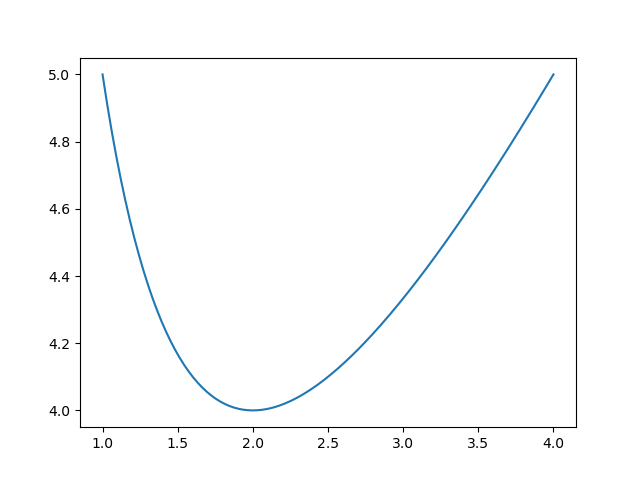
\includegraphics[width=0.70\linewidth]{figs/min.png}
    \caption{Plot of $f\brak{x} = x + \frac{4}{x}$ indicating the minimum at $\brak{2, 4}$}
    \label{fig:bt25_q14}
\end{figure}

\begin{lstlisting}[frame=single, basicstyle=\rmfamily, escapeinside={(*@}{@*)}]
(*@\makebox[\dimexpr\linewidth-2\fboxsep-2\fboxrule\relax][c]{codes/btq14/min.py}@*)
\end{lstlisting}

\begin{lstlisting}[frame=single, basicstyle=\rmfamily, escapeinside={(*@}{@*)}]
(*@\makebox[\dimexpr\linewidth-2\fboxsep-2\fboxrule\relax][c]{figs/min.png}@*)
\end{lstlisting}

\item Consider a nonlinear algebraic equation, $e^x - 2 = 0$. Using the Newton-Raphson method, with the initial guess of $x_0 = 1$, the approximated value of the root of the equation after one iteration is \underline{\hspace{1.5cm}} (round off to two decimal places).
\hfill (GATE~BT~2025)

\solution
The given objective function and its first derivative are:
\begin{align}
f\brak{x} &= e^x - 2 \\
f'\brak{x} &= e^x
\end{align}

Substituting $f\brak{x}$ and $f'\brak{x}$ into the Newton-Raphson recurrence relation from \eqref{eq:newton_raphson}:
\begin{align}
x_{n+1} &= x_n - \frac{e^{x_n} - 2}{e^{x_n}} \\
&= x_n - \brak{1 - \frac{2}{e^{x_n}}} \\
&= x_n - 1 + 2e^{-x_n}
\end{align}

Given the initial guess $x_0 = 1$, the first iteration ($n = 0$) gives:
\begin{align}
x_1 &= x_0 - 1 + 2e^{-x_0} \\
&= 1 - 1 + 2e^{-1} \\
&= \frac{2}{e} \approx \frac{2}{2.71828} \approx 0.73576 \approx 0.74
\end{align}

\noindent{Subsequent Iterations (Convergence to $\ln 2$):}
\begin{align}
x_2 &= x_1 - 1 + 2e^{-x_1} \approx 0.694042 \\
x_3 &= x_2 - 1 + 2e^{-x_2} \approx 0.693148 \\
x_4 &= x_3 - 1 + 2e^{-x_3} \approx 0.693147 \approx \ln 2
\end{align}

The exact mathematical solution is $e^x = 2 \implies x = \ln 2 \approx 0.693147$. Thus, the approximated value of the root after one iteration is ${0.74}$.

The C Code implementating Newton-Raphson recurrence is as follows: 
\begin{lstlisting}[frame=single, basicstyle=\rmfamily, escapeinside={(*@}{@*)}]
(*@\makebox[\dimexpr\linewidth-2\fboxsep-2\fboxrule\relax][c]{codes/btq33/raph.c}@*)
\end{lstlisting}

\begin{figure}[H]
    \centering
    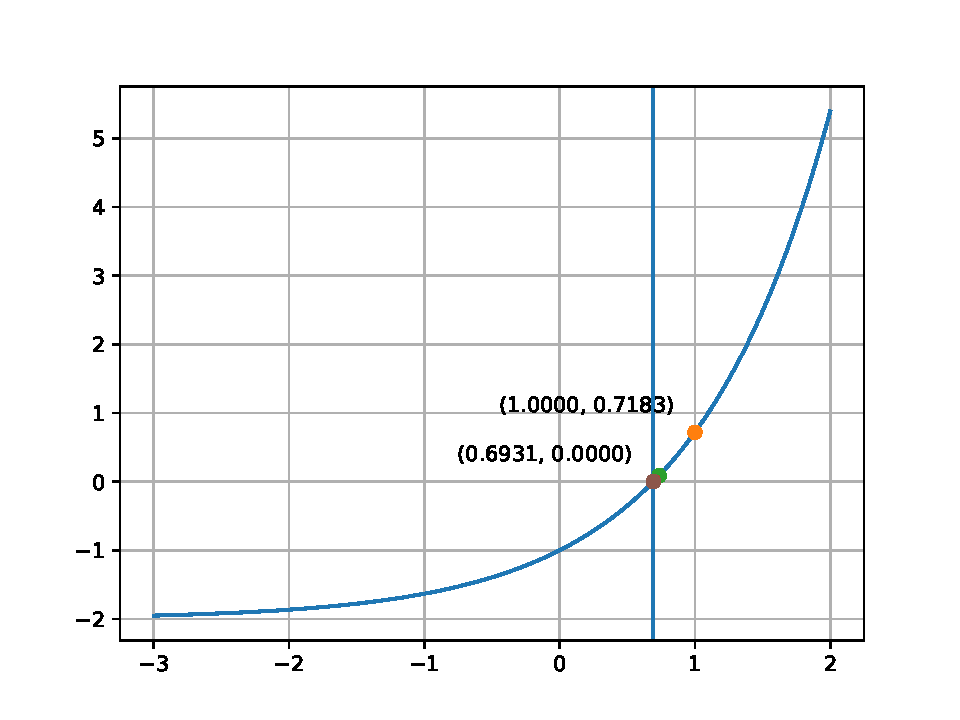
\includegraphics[width=0.70\linewidth]{figs/raph.pdf}
    \caption{Convergence of the Newton-Raphson method to $x = \ln 2$}
    \label{fig:bt25_q33}
\end{figure}

\begin{lstlisting}[frame=single, basicstyle=\rmfamily, escapeinside={(*@}{@*)}]
(*@\makebox[\dimexpr\linewidth-2\fboxsep-2\fboxrule\relax][c]{codes/btq33/raph.py}@*)
\end{lstlisting}

\item The value of $k$, for which the linear equations $2x + 3y = 6$ and $4x + 6y = 3k$ have at least one solution, is \underline{\hspace{1.5cm}} (answer in integer).
\hfill (GATE~BT~2025)

\solution
The given system of linear equations is:
\begin{align}
2x + 3y &= 6 \\
4x + 6y &= 3k
\end{align}
Expressing in matrix form $\vec{A}\vec{x} = \vec{b}$:
\begin{align}
\myvec{2 & 3 \\ 4 & 6} \myvec{x \\ y} = \myvec{6 \\ 3k}
\end{align}
The augmented matrix is formulated as:
\begin{align}
\augvec{2}{1}{\vec{A} & \vec{b}} = \augvec{2}{1}{2 & 3 & 6 \\ 4 & 6 & 3k}
\end{align}

Applying Gaussian elimination using the elementary row operation $R_2 \to R_2 - 2R_1$:
\begin{align}
\augvec{2}{1}{2 & 3 & 6 \\ 4 & 6 & 3k} \xrightarrow{R_2 \to R_2 - 2R_1} \augvec{2}{1}{2 & 3 & 6 \\ 0 & 0 & 3k - 12}
\end{align}
The coefficient matrix $\vec{A}$ reduces to:
\begin{align}
\vec{A} \xrightarrow{R_2 \to R_2 - 2R_1} \myvec{2 & 3 \\ 0 & 0}
\end{align}
Since there is only one non-zero row in echelon form, $\text{rank}\brak{\vec{A}} = 1$.

From the Rouch\'{e}--Capelli theorem in \eqref{eq:consistent_rank}, for the system to have at least one solution, it must be consistent:
\begin{align}
\text{rank}\brak{\augvec{2}{1}{\vec{A} & \vec{b}}} = \text{rank}\brak{\vec{A}} = 1
\end{align}
This requires the second row of the augmented matrix to be entirely zeros:
\begin{align}
3k - 12 &= 0 \\
3k &= 12 \implies k = 4
\end{align}
For $k = 4$, $\text{rank}\brak{\vec{A}} = \text{rank}\brak{\augvec{2}{1}{\vec{A} & \vec{b}}} = 1 < 2$ (number of variables $n = 2$), yielding infinitely many solutions along the coincident line $2x + 3y = 6$. 

Hence, the integer value of $k$ is ${4}$. \\


The Python Code showing the implementation for a given value of k and comparing solutions is as follows:
\begin{lstlisting}[frame=single, basicstyle=\rmfamily, escapeinside={(*@}{@*)}]
(*@\makebox[\dimexpr\linewidth-2\fboxsep-2\fboxrule\relax][c]{codes/btq34/bt34.py}@*)
\end{lstlisting}

\begin{figure}[H]
    \centering
    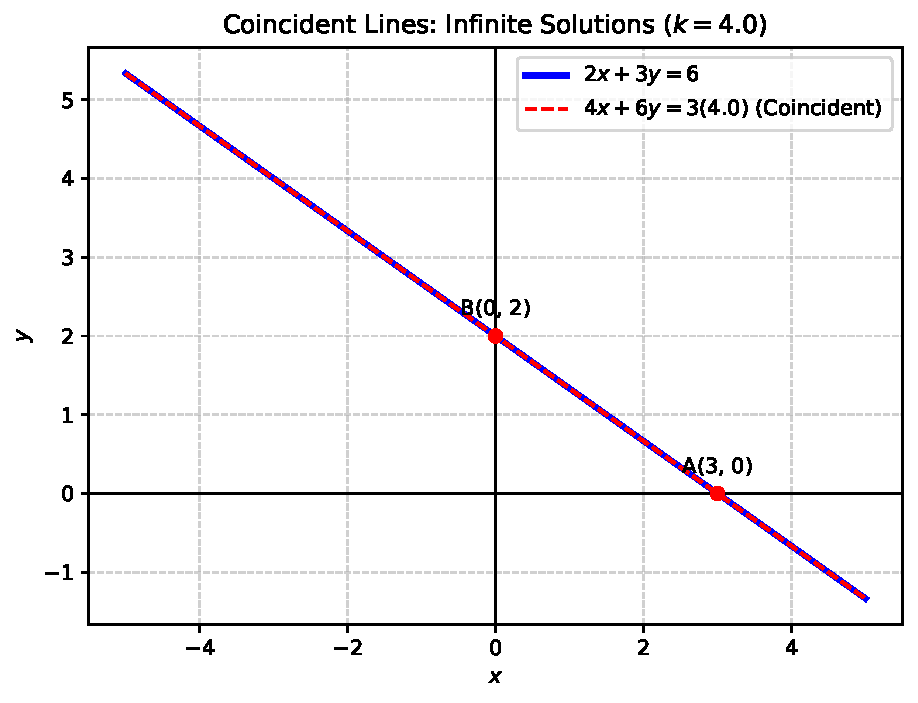
\includegraphics[width=0.70\linewidth]{figs/bt34_plot.pdf}
    \caption{Coincident lines representing infinitely many solutions at $k = 4$}
    \label{fig:bt25_q34}
\end{figure}

\item Two fair six-sided dice are rolled simultaneously. The probability that the sum of the numbers appearing on the top faces is $7$ is:
\hfill (GATE~BT~2025)
\begin{enumerate}
    \item $\frac{1}{6}$
    \item $\frac{5}{36}$
    \item $\frac{7}{36}$
    \item $\frac{1}{12}$
\end{enumerate}

\solution
Let $X_1$ and $X_2$ represent the scores on the two dice, and let $X = X_1 + X_2$ denote their sum. 

From the triangular distribution derived in \eqref{eq:triangular_pmf}, the probability mass function for $2 \le n \le 7$ is given by:
\begin{align}
p_X\brak{n} = \frac{n - 1}{36}
\end{align}

Evaluating the PMF at $n = 7$:
\begin{align}
p_X\brak{7} = \frac{7 - 1}{36} = \frac{6}{36} = \frac{1}{6}
\end{align}
Hence, option (A) is correct.

The Python simulation script verifying the PMF across 10,000 trials is:

\begin{lstlisting}[frame=single, basicstyle=\rmfamily, escapeinside={(*@}{@*)}]
(*@\makebox[\dimexpr\linewidth-2\fboxsep-2\fboxrule\relax][c]{codes/btq35/dice.py}@*)
\end{lstlisting}

\begin{figure}[H]
    \centering
    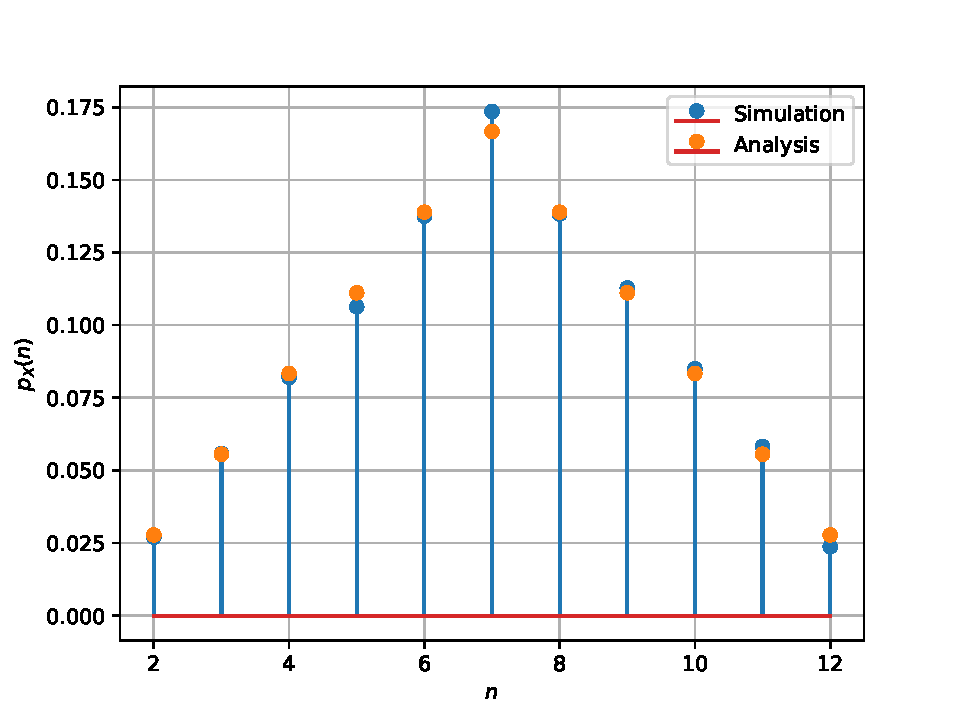
\includegraphics[width=0.70\linewidth]{figs/pmf.pdf}
    \caption{PMF of the sum of two fair dice: Simulation vs Analysis}
    \label{fig:bt25_q35}
\end{figure}

\begin{lstlisting}[frame=single, basicstyle=\rmfamily, escapeinside={(*@}{@*)}]
(*@\makebox[\dimexpr\linewidth-2\fboxsep-2\fboxrule\relax][c]{figs/pmf.pdf}@*)
\end{lstlisting}



\end{enumerate}
